\section{Results}
\label{sec:results}



In this section, we present the results of each research question.

\subsection{RQ1: In what context do developers use regular expressions?}
\label{rq1:survey}

The survey was completed by 18 professional software developers with an average of nine years of programming experience ($\sigma = 4.28$).
On average, survey participants report to compose 172 regexes per year ($\sigma$ = 250) and compose regexes on average once per month, with 28\% composing multiple regexes in a week and an additional 22\% composing regexes once per week. That is, 50\% of respondents uses regexes at least weekly.
Table~\ref{tab:regexenviron} shows how frequently participants compose regexes using each of several languages and technical environments.
Six (33\%) of the survey participants report to compose regexes using general purpose programming languages (e.g., Java, C, C\#) 1-5 times per year and five (28\%) do this 6-10 times per year.  Regexes were rarely used in query languages like SQL, but for command line usage in tools such as grep, 6 (33\%) participants use regexes 51+ times per year.

\newcommand{\horiz}{\hspace{2.1pt}}

\begin{table}
\caption{Survey results for number of regexes composed per year by technical environment (RQ1) \label{tab:regexenviron}}
\begin{center}
\begin{small}
\begin{tabular}{l | r @{  \horiz} r @{ \horiz } r @{ \horiz } r @{ \horiz } r @{ \horiz } r }
\toprule
\textbf{Language/Environment} & 0 & 1-5 & 6-10 & 11-20 & 21-50 & 51+ \\  \hline \bigstrut
General  (e.g., Java)  & 1 & 6 & 5 & 3& 1& 2 \\ \hline \bigstrut
Scripting  (e.g., Perl) &5 &4 &3 &3 &2  &1 \\ \hline \bigstrut
Query  (e.g., SQL) & 15&2 &0 &0 &1  & 0\\ \hline \bigstrut
Command line (e.g., grep)   &2 &5 &3 &2 &0  &6 \\ \hline \bigstrut
Text editor (e.g., IntelliJ)   & 2& 5& 0& 5& 1& 5\\
\bottomrule
\end{tabular}
\end{small}
\end{center}
\end{table}

\begin{table}
\caption{Survey results for regex usage frequencies for  activities, averaged using a 6-point likert scale: Very Frequently=6, Frequently=5, Occasionally=4, Rarely=3, Very Rarely=2, and Never=1 (RQ1)\label{tab:regexactivities}}
\begin{center}
\begin{small}
\begin{tabular}{l|c}
\toprule
\textbf{Activity} & \textbf{Frequency} \\  \hline \bigstrut
Locating content within a file or files & 4.4\\ \hline \bigstrut
Capturing parts of strings & 4.3 \\ \hline \bigstrut
Parsing user input & 4.0\\ \hline \bigstrut
Counting lines that match a pattern & 3.2\\ \hline \bigstrut
Counting  substrings that match a pattern & 3.2\\  \hline \bigstrut
Parsing generated text & 3.0\\  \hline \bigstrut
Filtering collections (lists, tables, etc.) & 3.0 \\ \hline \bigstrut
Checking for a single character & 1.7\\
\bottomrule
\end{tabular}
\end{small}
\end{center}
\end{table}

Table~\ref{tab:regexactivities} shows how frequently, on average, the participants use
regexes for various actives.
Participants answered questions using a 6-point likert scale including very frequently, frequently, occasionally, rarely, very rarely, and never.
Assigning values from 1 to 6, where 6 is the most frequent, the responses were averaged across participants.
Among the most common usages are capturing parts of a string and locating content within a file, with both occurring somewhere between occasionally and frequently.

Using a similar 7-point likert scale that includes `always' as a seventh point, developers indicated that they test their regexes with the same frequency as they test their code (average response was 5.2, which is between frequently and very frequently).  Half of the 18 developers indicate that they use external tools to test their regexes, and the other half indicated that they only use tests that they write themselves. Of the nine developers using tools, six mentioned some online composition aide such as \url{regex101.com} where a regex and input string are entered, and the input string is highlighted according to what is matched.
%The other three developers mentioned 'ScalaCheck' (a testing framework), 'IDE regex plugins', and 'Language specific Regexlib'.

When asked an open ended question about pain points encountered with regular expressions, we observed three main categories. The most common, ``hard to compose," was represented in 61\% (11) responses. Next,
 39\% (7) developers responded that regexes are ``hard to read" and 17\% (3) indicated difficulties with ``inconsistency across implementations," which manifest when using regexes in multiple languages. These responses do not sum to 18 as three developers provided overlapping  answers.

\paragraph{Summary - RQ1}
%The survey validates the assumption that regex are widely used by professional software developers and sheds some light into the context in which regexes are used.
%Future research into regex can focus on activities that prove to be most important to developers, namely capturing parts of strings and searching for specific content.
%Although research into regex use in general purpose and scripting languages is important, usage within command line tools and text editors should also be considered.

Overall, regexes are used frequently with common usages including locating content within a file, capturing parts of strings, and parsing user input.
The fact that all the surveyed developers compose regexes, and half of the developers use tools to test their regexes indicates the importance of tool development for regex.  Developers complain about regex being hard to read and hard to compose, and most of the tools that they indicate using are focused on composition.



\subsection{RQ2: How  is the {\tt re} module used?}
We explore regex utilizations and flags used in the scraped Python projects.
%We measure the frequency of usage for calls to the 8 functions of the {\tt re} module (i.e., {\tt compile}, {\tt search}, {\tt match}, {\tt split}, {\tt findall}, {\tt finditer}, {\tt sub} and {\tt subn}).
%We also measure usage of the 8 {\tt re} flags (i.e., {\tt DEFAULT}, {\tt IGNORECASE}, {\tt LOCALE}, {\tt MULTILINE}, {\tt DOTALL}, {\tt UNICODE}, {\tt VERBOSE} and {\tt DEBUG}).
%\subsubsection{Regex Utilizations per Project}
Out of the \DTLfetch{data}{key}{nProjScanned}{value}\ projects scanned, \DTLfetch{data}{key}{percentProjectsUsingRegex}{value}\% (\DTLfetch{data}{key}{nProjectsUsingRegex}{value}) contained at least one regex utilization.  To illustrate how saturated projects are with regexes, we measure utilizations per project, files scanned per project, files contained utilizations, and  utilizations  per file, as shown in Table~\ref{table:saturation}.

The average project contained 32 utilizations, and the maximum number of utilizations was 1,427.  The project with the most utilizations is a C\# project\footnote{\url{https://github.com/Ouroboros/Arianrhod}} that maintains a collection of source code for 20 Python libraries, including larger libraries like {\tt pip}, {\tt celery} and {\tt ipython}.  These larger Python libraries contain many utilizations.
From Table~\ref{table:saturation}, we also see that each project had an average of 11 files containing any utilization, and each of these files had an average of 2 utilizations.

% to find max nprojects: select distinct uniqueSourceID, count(*) as ct from RegexCitationMerged group by uniqueSourceID order by ct;


%As we scanned \DTLfetch{data}{key}{nProjScanned}{value} projects, we would expect to have seen $11*2*3898=85,756$ regex usages, which is higher than the actual \DTLfetch{data}{key}{nUsages}{value} usages observed. \todo{Explain why? Be pedantic. }

\begin{table}[tb]
\begin{center}
\begin{small}
\caption{How saturated are projects with utilizations? (RQ2)}
\label{table:saturation}

\begin{tabular}{l|ccccc}
\toprule
source & Q1 & Avg & Med & Q3 & Max \\ 
 \hline \bigstrut
utilizations per project & 2 & 32 & 5 & 19 & 1,427 \\ 
 \hline \bigstrut
files per project & 2 & 53 & 6 & 21 & 5,963 \\ 
 \hline \bigstrut
utilizing files per project & 1 & 11 & 2 & 6 & 541 \\ 
 \hline \bigstrut
utilizations per file & 1 & 2 & 1 & 3 & 207 \\ 
\bottomrule
\end{tabular}
\end{small}
\end{center}
\end{table}


%\subsubsection{Usage Frequency of {\tt re} Module}

\begin{figure}[tb]
\centering
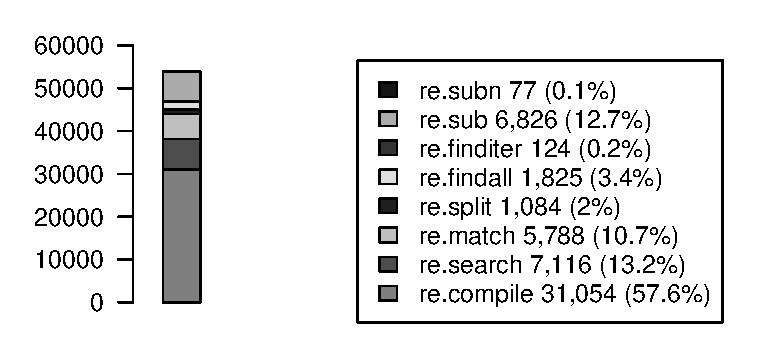
\includegraphics[width=\columnwidth]{../analysis_output/partFunctions.eps}
\vspace{-6pt}
\caption{How often are  {\tt re} functions used? (RQ2)}
\vspace{-6pt}
\label{fig:partFunctions}
\end{figure}

\begin{figure}[tb]
\centering
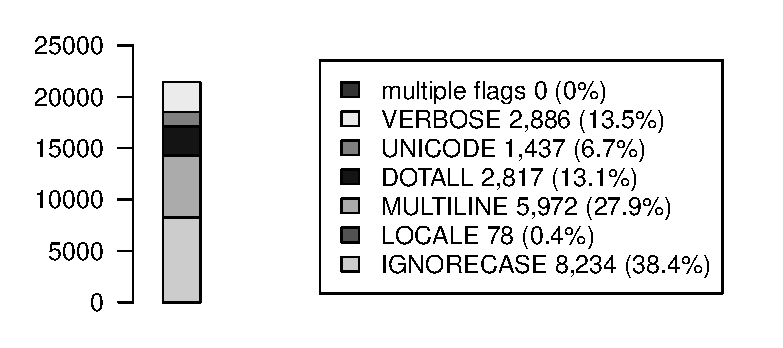
\includegraphics[width=0.9\columnwidth]{../analysis_output/partFlags.eps}
\vspace{-6pt}
\caption{Which behavioral flags are used? (RQ2)}
%\vspace{-6pt}
\label{fig:partFlags}
\end{figure}

\begin{table*}[h]
\begin{center}
\begin{small}
\caption{How Frequently do Features Appear in Projects? (RQ2)}
\label{table:featureStats}
\begin{tabular}
{ll@{ }llc@{ }c@{ }c@{ }ccccccc}
rank & code & description & example & brics & hampi & Rex & RE2 & nPatterns & \% patterns & nProjects & \% projects \\ 
\toprule[0.16em]
1 & ADD & one-or-more repetition & \begin{minipage}{0.5in}\begin{verbatim}z+\end{verbatim}\end{minipage} & \yes & \yes & \yes & \yes & 6,003 & 44.1 & 1,204 & 73.2 \\ 
\midrule
2 & CG & a capture group & \begin{minipage}{0.5in}\begin{verbatim}(caught)\end{verbatim}\end{minipage} & \yes & \yes & \yes & \yes & 7,130 & 52.4 & 1,194 & 72.6 \\ 
\midrule
3 & KLE & zero-or-more repetition & \begin{minipage}{0.5in}\begin{verbatim}.*\end{verbatim}\end{minipage} & \yes & \yes & \yes & \yes & 6,017 & 44.3 & 1,099 & 66.8 \\ 
\midrule
4 & CCC & custom character class & \begin{minipage}{0.5in}\begin{verbatim}[aeiou]\end{verbatim}\end{minipage} & \yes & \yes & \yes & \yes & 4,468 & 32.9 & 1,026 & 62.4 \\ 
\midrule
5 & ANY & any non-newline char & \begin{minipage}{0.5in}\begin{verbatim}.\end{verbatim}\end{minipage} & \yes & \yes & \yes & \yes & 4,657 & 34.3 & 1,005 & 61.1 \\ 
\midrule
6 & RNG & chars within a range & \begin{minipage}{0.5in}\begin{verbatim}[a-z]\end{verbatim}\end{minipage} & \yes & \yes & \yes & \yes & 2,631 & 19.3 & 848 & 51.6 \\ 
\midrule
7 & STR & start-of-line & \begin{minipage}{0.5in}\begin{verbatim}^\end{verbatim}\end{minipage} & \no & \yes & \yes & \yes & 3,563 & 26.2 & 846 & 51.4 \\ 
\midrule
8 & END & end-of-line & \begin{minipage}{0.5in}\begin{verbatim}$\end{verbatim}\end{minipage} & \no & \yes & \yes & \yes & 3,169 & 23.3 & 827 & 50.3 \\ 
\midrule[0.12em]
9 & NCCC & negated CCC & \begin{minipage}{0.5in}\begin{verbatim}[^qwxf]\end{verbatim}\end{minipage} & \yes & \yes & \yes & \yes & 1,935 & 14.2 & 776 & 47.2 \\ 
\midrule
10 & WSP & \textbackslash t \textbackslash n \textbackslash r \textbackslash v \textbackslash f or space & \begin{minipage}{0.5in}\begin{verbatim}\s\end{verbatim}\end{minipage} & \no & \yes & \yes & \yes & 2,846 & 20.9 & 762 & 46.3 \\ 
\midrule
11 & OR & logical or & \begin{minipage}{0.5in}\begin{verbatim}a|b\end{verbatim}\end{minipage} & \yes & \yes & \yes & \yes & 2,102 & 15.5 & 708 & 43 \\ 
\midrule
12 & DEC & any of: 0123456789 & \begin{minipage}{0.5in}\begin{verbatim}\d\end{verbatim}\end{minipage} & \no & \yes & \yes & \yes & 2,297 & 16.9 & 692 & 42.1 \\ 
\midrule
13 & WRD & [a-zA-Z0-9\_] & \begin{minipage}{0.5in}\begin{verbatim}\w\end{verbatim}\end{minipage} & \no & \yes & \yes & \yes & 1,430 & 10.5 & 650 & 39.5 \\ 
\midrule
14 & QST & zero-or-one repetition & \begin{minipage}{0.5in}\begin{verbatim}z?\end{verbatim}\end{minipage} & \yes & \yes & \yes & \yes & 1,871 & 13.8 & 645 & 39.2 \\ 
\midrule
15 & LZY & as few reps as possible & \begin{minipage}{0.5in}\begin{verbatim}z+?\end{verbatim}\end{minipage} & \no & \yes & \no & \yes & 1,300 & 9.6 & 605 & 36.8 \\ 
\midrule
16 & NCG & group without capturing & \begin{minipage}{0.5in}\begin{verbatim}a(?:b)c\end{verbatim}\end{minipage} & \no & \yes & \no & \yes & 791 & 5.8 & 404 & 24.6 \\ 
\midrule
17 & PNG & named capture group & \begin{minipage}{0.5in}\begin{verbatim}(?P<name>x)\end{verbatim}\end{minipage} & \no & \yes & \no & \yes & 915 & 6.7 & 354 & 21.5 \\ 
\midrule
18 & SNG & exactly n repetition & \begin{minipage}{0.5in}\begin{verbatim}z{8}\end{verbatim}\end{minipage} & \yes & \yes & \yes & \yes & 581 & 4.3 & 340 & 20.7 \\ 
\midrule
19 & NWSP & any non-whitespace & \begin{minipage}{0.5in}\begin{verbatim}\S\end{verbatim}\end{minipage} & \no & \yes & \yes & \yes & 484 & 3.6 & 270 & 16.4 \\ 
\midrule
20 & DBB & $n\le x \le m$ repetition & \begin{minipage}{0.5in}\begin{verbatim}z{3,8}\end{verbatim}\end{minipage} & \yes & \yes & \yes & \yes & 367 & 2.7 & 238 & 14.5 \\ 
\midrule
21 & NLKA & sequence doesn't follow  & \begin{minipage}{0.5in}\begin{verbatim}a(?!yz)\end{verbatim}\end{minipage} & \no & \no & \no & \no & 131 & 1 & 183 & 11.1 \\ 
\midrule
22 & WNW & word/non-word boundary & \begin{minipage}{0.5in}\begin{verbatim}\b\end{verbatim}\end{minipage} & \no & \no & \no & \yes & 248 & 1.8 & 166 & 10.1 \\ 
\midrule
23 & NWRD & non-word chars & \begin{minipage}{0.5in}\begin{verbatim}\W\end{verbatim}\end{minipage} & \no & \yes & \yes & \yes & 94 & 0.7 & 165 & 10 \\ 
\midrule
24 & LWB & at least n repetition & \begin{minipage}{0.5in}\begin{verbatim}z{15,}\end{verbatim}\end{minipage} & \yes & \yes & \yes & \yes & 91 & 0.7 & 158 & 9.6 \\ 
\midrule
25 & LKA & matching sequence follows & \begin{minipage}{0.5in}\begin{verbatim}a(?=bc)\end{verbatim}\end{minipage} & \no & \no & \no & \no & 112 & 0.8 & 158 & 9.6 \\ 
\midrule
26 & OPT & options wrapper & \begin{minipage}{0.5in}\begin{verbatim}(?i)CasE\end{verbatim}\end{minipage} & \no & \yes & \no & \yes & 231 & 1.7 & 154 & 9.4 \\ 
\midrule
27 & NLKB & sequence doesn't precede & \begin{minipage}{0.5in}\begin{verbatim}(?<!x)yz\end{verbatim}\end{minipage} & \no & \no & \no & \no & 94 & 0.7 & 137 & 8.3 \\ 
\midrule[0.12em]
28 & LKB & matching sequence precedes & \begin{minipage}{0.5in}\begin{verbatim}(?<=a)bc\end{verbatim}\end{minipage} & \no & \no & \no & \no & 80 & 0.6 & 120 & 7.3 \\ 
\midrule
29 & ENDZ & absolute end of string & \begin{minipage}{0.5in}\begin{verbatim}\Z\end{verbatim}\end{minipage} & \no & \no & \no & \yes & 89 & 0.7 & 90 & 5.5 \\ 
\midrule
30 & BKR & match the $i^{th}$ CG & \begin{minipage}{0.5in}\begin{verbatim}\1\end{verbatim}\end{minipage} & \no & \no & \no & \no & 60 & 0.4 & 84 & 5.1 \\ 
\midrule
31 & NDEC & any non-decimal & \begin{minipage}{0.5in}\begin{verbatim}\D\end{verbatim}\end{minipage} & \no & \yes & \yes & \yes & 36 & 0.3 & 58 & 3.5 \\ 
\midrule
32 & BKRN & references PNG & \begin{minipage}{0.5in}\begin{verbatim}\g<name>\end{verbatim}\end{minipage} & \no & \yes & \no & \no & 17 & 0.1 & 28 & 1.7 \\ 
\midrule
33 & VWSP & matches U+000B & \begin{minipage}{0.5in}\begin{verbatim}\v\end{verbatim}\end{minipage} & \no & \no & \yes & \yes & 13 & 0.1 & 15 & 0.9 \\ 
\midrule
34 & NWNW & negated WNW & \begin{minipage}{0.5in}\begin{verbatim}\B\end{verbatim}\end{minipage} & \no & \no & \no & \yes & 4 & 0 & 11 & 0.7 \\ 
\bottomrule[0.13em]
\end{tabular}
\end{small}
\end{center}
\vspace{-12pt}
\end{table*}


The number of projects that use each of the {\tt re} functions is shown in Figure~\ref{fig:partFunctions}.  The y-axis denotes the total utilizations, with a maximum of \DTLfetch{data}{key}{nUsages}{value}. The {\tt re.compile} function encompasses \DTLfetch{data}{key}{percentCompile}{value}\% of all utilizations, presumably because each usage of those functions can accept a regex object compiled using {\tt re.compile} as an argument.
%\todoNow{can we connect any of these function calls to the findings from the survey? For example, according to Table~\ref{tab:regexactivities}, participants frequently or occasionally want to capture parts of strings, which maps to the X function in {\tt re}}
%\subsubsection{Usage Frequency of {\tt re} Module Flags}

When considering flag use, we excluded the default flag, which is built into the {\tt re} module, and present internally whenever no flag is used.  Of all utlizations, \DTLfetch{data}{key}{percentFlags0}{value}\% had no flag, or explicitly specified the default flag.  The debug flag, which causes the {\tt re} regex engine to display extra information about its parsing process, was never observed.
 Figure~\ref{fig:partFlags} presents the number of projects in which each flag appears. Ignorecase (\DTLfetch{data}{key}{percentI}{value}\%) and multiline (\DTLfetch{data}{key}{percentM}{value}\%) were the most frequently used.   Although multiple flags can be combined using a bitwise or, this was never observed.



%\subsubsection{Most Frequently Observed Patterns}
%
%Table~\ref{table:topNW} contains the most frequently used patterns, ordered by the number of projects in which the pattern appears.  \todoNow{Is this still true???} The patterns are quoted to show the presence of spaces, if any.  We  elaborate on the top four patterns and  reference the feature set in Table~\ref{table:featureStats}.
%
%
%The first pattern, \verb!`\s+'!, uses the WSP character class feature.  This character class represents one or more whitespace characters,  defined as spaces, tabs, newlines, vertical whitespace, carriage returns or form feeds.  The \verb!+! (the ADD feature) at the end of the pattern means that it must match one or more whitespace characters.  The pattern \verb!`\s+'! is often used to split sentences into separate words which may have more than one space between them, or contain tabs or other types of whitespace.
%
%Interestingly, the second most common pattern, \verb!`\s'!, also uses the WSP character. In this case, it does not match several whitespace characters (though it would match the first of several).
%
%The third pattern, \verb!\d+!,  uses the DEC character class, which is composed of the digits from 0 to 9.  Like the first pattern, the third uses the ADD feature to match one or more digits.
%
%The fourth pattern, \verb![\x80-\xff]!, uses the CCC feature to create a custom character class, and the RNG feature to specify a range of characters.
%%The hexadecimal value \verb!\x80! is equivalent to the value 128 in decimal, and the hexadecimal value \verb!\xff! is equivalent to 255 in decimal.
%When hexadecimal values are used within a character class like this (and the UNICODE flag is not active), it signifies the corresponding characters in an ASCII lookup table.
%%The range specified by this pattern is highlighted on the right side of Figure~\ref{fig:ASCIItable}.  Table image found at: \url{https://courses.engr.illinois.edu/ece390/books/labmanual/ascii-code/quickref.png}.
%%\todo{run program again to unescape pattern strings}
%%\todo{Figure 6 seems largely unnecessary}
%
%
%%\todo{more of the topN patterns if there is space}
%
%%\begin{figure}[tb]
%%\centering
%%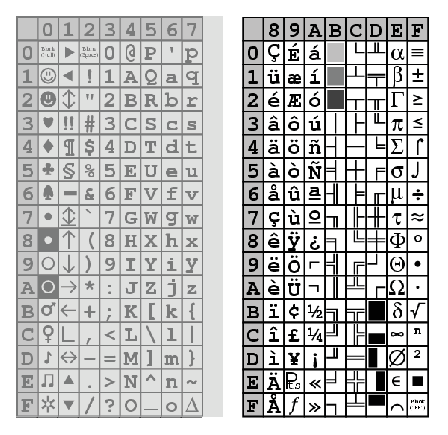
\includegraphics[width=\columnwidth]{../illustrations/ASCIItable.eps}
%%\cprotect\caption{On the Right, ASCII Characters Matching \verb!'[\x80-\xff]'! (RQ1)}
%%\label{fig:ASCIItable}
%%\end{figure}
%
%\begin{table}
\caption{ \label{}}
\begin{center}
\begin{tabular}{lc}
\toprule
pattern & weight \\ 
\midrule
\begin{minipage}{2.3in}
\begin{verbatim}
'\\s+'\end{verbatim}
\end{minipage}
& 181 \\ 
\midrule
\begin{minipage}{2.3in}
\begin{verbatim}
'\\s'\end{verbatim}
\end{minipage}
& 78 \\ 
\midrule
\begin{minipage}{2.3in}
\begin{verbatim}
'\\d+'\end{verbatim}
\end{minipage}
& 70 \\ 
\midrule
\begin{minipage}{2.3in}
\begin{verbatim}
'[\\x80-\\xff]'\end{verbatim}
\end{minipage}
& 69 \\ 
\midrule
\begin{minipage}{2.3in}
\begin{verbatim}
'\nmd5_data = {\n([^}]+)}'\end{verbatim}
\end{minipage}
& 69 \\ 
\midrule
\begin{minipage}{2.3in}
\begin{verbatim}
'\\\\(.)'\end{verbatim}
\end{minipage}
& 67 \\ 
\midrule
\begin{minipage}{2.3in}
\begin{verbatim}
'([\\\\"]|[^\\ -~])'\end{verbatim}
\end{minipage}
& 66 \\ 
\midrule
\begin{minipage}{2.3in}
\begin{verbatim}
'(-?(?:0|[1-9]\\d*))(\\.\\d+)?([eE][-+]?\\d+)?'\end{verbatim}
\end{minipage}
& 61 \\ 
\midrule
\begin{minipage}{2.3in}
\begin{verbatim}
'[^]]+?\\] +([0-9.]+): (\\w+) <-(\\w+)'\end{verbatim}
\end{minipage}
& 60 \\ 
\midrule
\begin{minipage}{2.3in}
\begin{verbatim}
'.*rlen=([0-9]+)'\end{verbatim}
\end{minipage}
& 57 \\ 
\bottomrule
\end{tabular}
\end{center}
\end{table}


% %\subsection{Pattern Characteristics}

% Table~\ref{table:patternStats} (description of table contents)

% \begin{table}[tb]
\begin{center}
\caption{Pattern Characteristics (RQ1)}
\label{table:patternStats}

\begin{tabular}{l|ccccc}
\toprule
source & Q1 & Avg & Med & Q3 & Max \\ 
\midrule
pattern weight & 1 & 2 & 1 & 2 & 182 \\ 
\midrule
token count & 8 & 23 & 14 & 24 & 31,349 \\ 
\midrule
distinct features & 3 & 5 & 5 & 7 & 20 \\ 
\midrule
pattern length & 13 & 37 & 22 & 38 & 43,255 \\ 
\bottomrule
\end{tabular}
\end{center}
\end{table}

%\todoNow{add patternStats table back in and describe it if there is enough time.  Note the longest pattern present in patternLength.csv in analysis folder was probably automatially generated from text and is monstrous!}


\paragraph{Summary - RQ2}

Only about half of the projects sampled contained any utilizations.  Most utilizations used the {\tt re.compile} function to compile a regex object before actually using the regex to find a match.  Most utilizations did not use a flag to modify matching behavior.




%The most frequently observed patterns were used to match whitespace and digits.

\subsection{RQ3: Which regular expression language features are most commonly used in Python?}
\label{results:rq3}

To measure feature usage, we  count the number of usages of each feature per project and as a percent of all distinct regular expression patterns in the corpus.



\subsubsection{Feature Usage}
\label{sec:featureUsage}
Table~\ref{table:featureStats} displays feature usage from the corpus and relates it to four major regex related projects. Only features appearing in at least 10 projects are listed.
The first column, \emph{rank}, lists the rank of a feature (relative to other features) in terms of the number of projects in which it appears. The next column, \emph{code}, gives a succinct reference string for the feature, and is followed by a \emph{description} column that provides a brief comment on what the feature does.  The \emph{example} column provides a short example of how the feature can be used.
% For example, the most common feature observed in the corpus is \emph{one-or-more repetition}, which is specified in a pattern by using the {\tt +} character in conjunction with some sub-pattern that should repeat one or more times.  The code for this feature is \emph{ADD}, and the short example provided is \verb!z+!.
The next four columns, (i.e., \emph{brics}, \emph{hampi}, \emph{Rex}, and \emph{RE2}), map to the four major research projects chosen for our investigation (see Section~\ref{regextoolsresults}).  We indicate that a project supports a feature with the `\yes' symbol, and indicate that a project does not support the feature with the `\no' symbol.
The final four columns contain two pairs of usage statistics.  The first pair contains the number and percent of \emph{patterns} that a feature appears in, out of the 13,912 patterns that make up the corpus.  The second pair of columns contain the number and percent of \emph{projects} that a feature appears in out of the 1645 projects scanned that contain at least one utilization.

One notable omission from Table~\ref{table:featureStats} is the literal feature, which is used  to specify matching any specific character.  An example pattern that contains only one literal token is the pattern \verb!`a'!.  This pattern only matches the lowercase letter `a'.  The literal feature was found in \DTLfetch{data}{key}{P_LITERAL_PRESENT}{value}\% of patterns.
%, and accounted for \DTLfetch{data}{key}{P_LITERAL_TOKENS}{value}\% of all tokens.
We consider the literal feature to be ubiquitous in all patterns, and necessary for any regex related tool to support, and so exclude it from Table~\ref{table:featureStats} and the rest of the feature analysis.



The eight most commonly used features, ADD, CG, KLE, CCC, ANY, RNG, STR and END,
appear in over half the projects. %The remaining 26 features appear in less than half of the projects containing utilizations.
CG is more commonly used in patterns than the highest ranked feature (ADD) by a wide margin (over 8\%), even though they appear in similar numbers of projects.

\subsubsection{Feature Support in Regex Tools}
\label{regextoolsresults}
While there are many regex tools available, in this work, we focus on the features support for these four tools, brics, hampi, Rex and RE2, which offer diversity across developers (i.e., Microsoft, Google, open source, and academia) and across applications. Further, as we wanted to perform a feature analysis, these four tools and their features are well-documented, allowing for easy comparison.

% We  mapped the features from the corpus to those features supported by the four regular expression engines described in Section~\ref{sec:related}: brics, hampi, RE2, and Rex.
To create the tool mappings, we consulted documentation for each of the selected regular expression engines. For brics, we collected the set of supported features using the formal grammar\footnote{\url{http://www.brics.dk/automaton/doc/index.html?dk/brics/automaton/RegExp.html}}.  For hampi, we manually inspected the set of regexes included in the {\tt lib/regex-hampi/sampleRegex} file within the hampi repository\footnote{\url{https://code.google.com/p/hampi/downloads/list}} (this may have been an overestimation, as this included more features than specified by the formal grammar\footnote{\url{http://people.csail.mit.edu/akiezun/hampi/Grammar.html}}).  For RE2, we used the  supported feature documentation\footnote{\url{https://re2.googlecode.com/hg/doc/syntax.html}}.  For Rex, we collected the feature set empirically because we tried to parse all patterns with Rex for the semantic analysis (Section~\ref{rq4:results}), and Rex provides comprehensive error feedback for unsupported features.

%\todoLast{Were there any features supported by the tools that we did not find in the corpus? Answer: RE2 has a lot of features we didn't study and that weren't found in the corpus in any substantial quantity.  I think this is addressed by the earlier mention: Only features appearing in at least 10 projects are listed.}


Of the four projects selected for this analysis, RE2 supports the most studied features (28 features) followed by hampi (25 features),  Rex (21 features), and brics (12 features).  All projects support the 8 most commonly used features except brics, which does not support STR or END.
%All projects support NCC, OR, and the four less common repetition features: QST, SNG, DBB and LWB.  RE2 is the only project to support the WNW, ENDZ and NWNW features.
No projects support the four look-around features LKA, NLKA, LKB and NLKB.  RE2 and hampi support the LZY, NCG, PNG and OPT features, whereas brics and Rex do not.%, which inspired in part the survey questions about feature usage.


\subsubsection{Survey Results for Feature Usage}
The pattern language for Python, which is used to compose regexes, supports default character classes like the ANY or dot character class: \verb!.! meaning, `any character except newline' (a full list of features and examples is in the first four columns of Table~\ref{table:featureStats}).
It also supports three other default character classes: \verb!\d!, \verb!\w!, \verb!\s! (and their negations). All of these default character classes can be simulated using the custom character class (CCC) feature, which can create semantically equivalent regexes.
For example  the decimal character class: \verb!\d! is equivalent to a CCC containing all 10 digits:  \verb!\d! $\equiv$ \verb![0123456789]! $\equiv$ \verb![0-9]!.
%Users have a choice when using regex between writing \verb!\d! and \verb![0-9]! and whereas the first option may be shorter, the second may seem more intuitive and readable.
Other default character classes such as the word character class: \verb!\w! may not be as intuitive to encode in a CCC: \verb![a-zA-Z0-9_]!.

Survey participants were asked if they use only CCC, use CCC more than default, use both equally, use default more than CCC or use only default.  Results for this question are shown in Table~\ref{tab:cccvsdefault}, with 67\% (12) indicating that they use default the most.
Participants were also asked to explain their preferences.  Participants who favored CCC mostly said something equivalent to ``it is more explicit," whereas the participants who favored default character classes said,  ``it is less verbose" and ``I like using built-in code."

\begin{table}
\caption{Survey results for preferences between custom character and default character classes (RQ3) \label{tab:cccvsdefault}}
\begin{center}
\begin{small}
\begin{tabular}{l|c}
\toprule
\textbf{Preference} & \textbf{Frequency} \\  \hline \bigstrut
use only CCC & 1\\ \hline \bigstrut
use CCC more than default & 5 \\ \hline \bigstrut
use both equally & 2\\ \hline \bigstrut
use default more than CCC & 10\\ \hline \bigstrut
use only default & 2\\
\bottomrule
\end{tabular}
\end{small}
\end{center}
\end{table}

To further explore how frequently participants use various regex features, participants were asked five questions (on a 6-point likert scale) about how frequently they use specific related groups of features,
%\begin{itemize} \itemsep -2pt
%    \item endpoint anchors (STR, END): \verb!^! and \verb!$!
%    \item capture groups(CG): (capture me)
%    \item word boundaries (WNW): \verb!word\b!
%    \item (negative) look-ahead/behinds (LKA, NLKA, LKB, NLKB): \verb!a(?=bc)!, \verb!(?<!x)yz!, \verb!(?<=a)!, \verb!a(?!yz)!
%    \item lazy repetition (LZY): \verb!ab+?!, \verb!xy{2,3}?!
%\end{itemize}
%These features were
chosen based on the tool feature support explored in Section~\ref{regextoolsresults}.
Results are shown in Table~\ref{tab:regexfeaturegroups}, indicating that lazy repetition and look-ahead features are rarely used and capture groups and endpoint anchors are occasionally to frequently used.


\begin{table}
\caption{Survey results for regex usage frequencies, averaged using a 6-point likert scale: Very Frequently=6, Frequently=5, Occasionally=4, Rarely=3, Very Rarely=2, and Never=1 (RQ3) \label{tab:regexfeaturegroups}}
\begin{center}
\begin{small}
\begin{tabular}{llc}
\toprule
\textbf{Group} & \textbf{Code} &  \textbf{Frequency} \\  \hline \bigstrut
endpoint anchors & (STR, END) & 4.4\\ \hline \bigstrut
capture groups & (CG) & 4.2 \\ \hline \bigstrut
word boundaries & (WNW) & 3.5 \\ \hline \bigstrut
lazy repetition & (LZY) &  2.9\\ \hline \bigstrut
\multirow{2}{*}{(neg) look-ahead/behind} &  (LKA, NLKA,  & \multirow{2}{*}{2.5}\\
& LKB, NLKB) & \\
\bottomrule
\end{tabular}
\end{small}
\end{center}
\end{table}




\paragraph{Summary - RQ3}
We found that the eight most common features are found on over 50\% of the projects.
We also identify brics as the project supporting the fewest features and RE2 as the project supporting the most features, and identify groups of features supported or not supported by the four regex projects. Some of the less supported features, such as endpoint anchors and capture groups, are used by developers occasionally to frequently.
%I was confused by the 'at least occasionally' verbage, at first it looked like 'the least occasionally'

From Table~\ref{table:featureStats} we know that STR and END features are present in over half of the scanned projects containing utilizations.  In our survey, over half (56\%) of the respondents answers that they use endpoint anchors frequently or very frequently, and none of them claimed to never use them. The brics library does not support this feature, which is a missed opportunity for developers who could otherwise have used brics to model their regexes that use STR and END.

The LZY feature  is present in over 36\% of scanned projects with utilizations (Table~\ref{table:featureStats}), and yet was not supported by two of the four major regex projects we explored, brics and RE2.
In our developer survey, 11\% (2) of participants use this feature frequently and 6 (33\%) use it occasionally, showing a modest impact on potential users.

%\subsubsection{PNG and BKRN vs CG and BKR}
%The PNG group (python-style named capture groups) and BKRN (back-references: named) are intended to operate together to allow users to name the content that is expected to appear in a capture group.  A simple example of how these can be used together with the named capture group matching some vowel is:
%\verb!(?P<vowel>[aeiou]x(?P=vowel))! which will match the strings 'axa' and 'oxo' but not 'txt'.  The same functionality can be obtained with a much shorter expression: \verb!([aeiou])x\1! where the \verb!'\1'! references the CG started by the first left parenthesis found when moving from left to right.
When survey participants were asked if they prefer to always use numbered (BKR) or named (BKRN) back references, 66\% (12) of survey participants said that they always use BKR, and the remaining 33\% (6) said ``it depends."  Not one participant preferred named capture groups.  BKR is present in 5\% of scanned projects, while BKRN is present in only 1.7\%, which corroborates our findings that numbered  are generally preferred over named capture groups.

\subsection{RQ4: How behaviorally similar are regexes?}
\label{rq4:results}


In clustering the regular expressions, we are interested in observing cross-project regex similarity and thus discarded patterns found in only one project.
Since Rex does not support all the regex features present in the corpus, we only generated sets of strings for measuring similarity for 2,871 (21\%) of the \DTLfetch{data}{key}{nCorpus}{value} patterns in the corpus. The impact is that 923 projects were excluded from the data set for the similarity analysis. Omitted features are indicated in Table~\ref{table:featureStats}, as described in Section~\ref{results:rq3}.
The generated strings for each pattern are used to measure the pairwise similarity for all patterns and construct the similarity matrix.


%\subsubsection{Rationale for Behavioral Clustering}
When tool designers are considering what features to include, data about usage in practice is valuable.  Semantic similarity clustering  helps to discern these behaviors by looking beyond the structural details of specific patterns and seeing trends in actual matching behavior.  We are also able to find out what features are being used in these behavioral trends so that we can make assertions about why certain features are important.

%\subsubsection{General Information About Clusters Found}
From 2,871 distinct patterns, the MCL clustering technique identified 186 clusters with 2 or more patterns, and 2,042 clusters of size 1.  Recall that only pairs of patterns with a similarity level of 0.75 were included in the matrix passed to MCL.  The average size of clusters larger than size one was 4.5.  Each pattern belongs to exactly one cluster.

%\subsubsection{An Example Cluster}
Table~\ref{table:exampleCluster} provides an example of a behavioral cluster containing 12 patterns (4 longer patterns omitted for brevity) with at least one pattern from this cluster present in 31 different projects.  All patterns in this cluster share the literal `:' character.
%Three example strings generated by Rex for the first pattern are: `-()', `*'8(5)', `Oe()'.  For the third pattern, Rex generated these three strings: ` ()', `(q)F', `(n)M'.  The pattern: \verb!\(.*\)$! is very similar, but will not match the string `(n)M', and so was placed in a different cluster.

\begin{table}
\begin{center}
\caption{Sample from an example cluster (RQ4)}
\label{table:exampleCluster}
\begin{small}
\begin{tabular}
{lcc | lcc}
\toprule
index & pattern & nProjects & index & pattern & nProjects \\
 \hline \bigstrut
1 & \begin{minipage}{0.3in}\begin{verbatim}`:+'\end{verbatim}\end{minipage} & 8 & 5 & \begin{minipage}{0.5in}\begin{verbatim}`[:]'\end{verbatim}\end{minipage} & 6 \\
 \hline \bigstrut
2 & \begin{minipage}{0.3in}\begin{verbatim}`(:)'\end{verbatim}\end{minipage} & 8 & 6 & \begin{minipage}{0.6in}\begin{verbatim}`([^:]+):(.*)'\end{verbatim}\end{minipage} & 6 \\
 \hline \bigstrut
3 & \begin{minipage}{0.3in}\begin{verbatim}`(:+)'\end{verbatim}\end{minipage} & 8 & 7 & \begin{minipage}{0.5in}\begin{verbatim}`\s*:\s*'\end{verbatim}\end{minipage} & 4 \\
 \hline \bigstrut
4 & \begin{minipage}{0.3in}\begin{verbatim}`(:)(:*)'\end{verbatim}\end{minipage} & 8 & 8 & \begin{minipage}{0.5in}\begin{verbatim}`\:'\end{verbatim}\end{minipage} & 2 \\
\bottomrule
\end{tabular}
\vspace{-6pt}
\end{small}
\end{center}
\end{table}


%
%\begin{table}
%\begin{center}
%\caption{An example cluster (RQ3)}
%\label{table:exampleCluster}
%\begin{small}
%\begin{tabular}
%{lcc}
%\toprule
%index & pattern & nProjects\\
%\midrule
%1 & \begin{minipage}{0.5in}\begin{verbatim}`\s*,\s*'\end{verbatim}\end{minipage} & 54  \\
%\midrule
%2 & \begin{minipage}{0.5in}\begin{verbatim}`,'\end{verbatim}\end{minipage} & 30 \\
%\midrule
%3 & \begin{minipage}{0.5in}\begin{verbatim}`\s*,'\end{verbatim}\end{minipage} & 16 \\
%\midrule
%4 & \begin{minipage}{0.5in}\begin{verbatim}` ,\s*'\end{verbatim}\end{minipage} & 13 \\
%\midrule
%5 & \begin{minipage}{0.5in}\begin{verbatim}` *, *'\end{verbatim}\end{minipage} & 12 \\
%\midrule
%6 & \begin{minipage}{0.5in}\begin{verbatim}`,\S'\end{verbatim}\end{minipage} & 5 \\
%\midrule
%7 & \begin{minipage}{0.5in}\begin{verbatim}`,.*$'\end{verbatim}\end{minipage} & 3 \\
%\midrule
%8 & \begin{minipage}{0.6in}\begin{verbatim}`(\S+)\s*,\s*'\end{verbatim}\end{minipage} & 2 \\
%\midrule
%9 & \begin{minipage}{0.5in}\begin{verbatim}`,+'\end{verbatim}\end{minipage} & 1 \\
%\midrule
%10 & \begin{minipage}{0.5in}\begin{verbatim}`,\ ?'\end{verbatim}\end{minipage} & 1 \\
%\midrule
%10 & \begin{minipage}{0.5in}\begin{verbatim}`,\s*(\S)'\end{verbatim}\end{minipage} & 1 \\
%\midrule
%11 & \begin{minipage}{0.5in}\begin{verbatim}`\s*(,)\s*'\end{verbatim}\end{minipage} & 1 \\
%\midrule
%12 & \begin{minipage}{0.5in}\begin{verbatim}`\s*\,\s*'\end{verbatim}\end{minipage} & 1 \\
%\bottomrule
%\end{tabular}
%\end{small}
%\end{center}
%\end{table}


%\subsubsection{Using the Smallest Pattern to Represent a Cluster}
The smallest pattern in Table~\ref{table:exampleCluster} contains only the colon and the plus character \verb!`:+'! at index 1.  This smallest pattern gives a good idea of what all the patterns within the cluster have in common.  A shorter pattern will tend to have less extraneous behavior because it is specifying less behavior.  And yet in order for the smallest pattern to be clustered with other patterns, it had to match most of the strings created by Rex from another pattern within the cluster, and so we assume that \emph{the smallest pattern is a good representation of the cluster}.

For the rest of this paper, a cluster will be represented by one of the shortest patterns it contains, followed by the number of projects any member of the cluster appears in, so the cluster in Table~\ref{table:exampleCluster} will be represented as \verb!`:+'(31)!.

We manually mapped the top 100 clusters into 6 behavioral categories (determined by inspection).  The largest cluster was left out, as it was composed of patterns that trivially matched almost any string, like \verb!`b*'! and \verb!`^'!.  The remaining 99 clusters were all categorized.

When a cluster can fit in multiple categories, it is placed in the most specific category.  The following six categories are listed in order from most specific behavior to least specific behavior.

\begin{table}
\begin{center}
\begin{small}
\caption{Cluster categories and sizes (RQ4) \label{tab:clustercats}}
\begin{tabular}{llll}
\toprule
\textbf{Category} & \textbf{Clusters} & \textbf{Patterns} & \textbf{Projects} \\  \hline \bigstrut
Code Search & 15 & 27 & 92 \\ \hline \bigstrut
Content of Parens & 10 & 46 & 111\\ \hline \bigstrut
Anchored Patterns & 20 & 85 & 141\\ \hline \bigstrut
Two or More Chars & 16 & 40 & 120\\ \hline \bigstrut
Requiring a Char & 17 & 103 & 184\\ \hline \bigstrut
Multi Matches & 21 & 237 & 295\\
\bottomrule
\end{tabular}
\end{small}
\end{center}
\end{table}

\subsubsection{Code Search and Variable Capturing}
This category contains 15 clusters, each appearing in an average of 11.7 projects.  These clusters have a combined total of 27 patterns, with at least one pattern present in 92 projects. These clusters center around a recognizable effort to parse code and often capture variable values in it, for example:
\verb!`^https?://'(23)!, \verb!`(.+)=(.+)'(9)!, \verb!`\$\{([\w\-]+)\}'(11)!, and \verb!`SECRET|PASSWORD|PROFANITIES_LIST'(13)!

\subsubsection{Content Of Brackets and Parenthesis}
This category contains 10 clusters, each appearing in an average of 18.4 projects.  These clusters have a combined total of 46 patterns, with at least one pattern present in 111 projects. Each of the clusters center around finding a pair of characters that surround content, often capturing that content:
\verb!`\(.*\)'(29)!, \verb!`".*"'(25)!, \verb!`<(.+)>'(23)!, and \verb!`\[.*\]'(22)!.

\subsubsection{Anchored Patterns}
This category contains 20 clusters, each appearing in an average of 15.4 projects.  These clusters have a combined total of 85 patterns, with at least one pattern present in 141 projects. Each of the clusters uses at least one endpoint anchor to require matches to be absolutely positioned, for example:
\verb!`(\w+)$'(35)!, \verb!`^-?\d+$'(17)!, \verb!`^\s'(16)!, and \verb!`^[ -~]*$'(10)!.

\subsubsection{Requiring Two or More Characters in Sequence}
This category contains 16 clusters, each appearing in an average of 13 projects.  These clusters have a combined total of 40 patterns, with at least one pattern present in 120 projects. These clusters require several characters in a row to match some pattern, for example:
\verb!`\d+\.\d+'(30)!, \verb!`  '(17)!, \verb!`([A-Z][a-z]+[A-Z][^ ]+)'(11)!, and \verb!@[a-z]+'(9)!.

\subsubsection{Requiring a Specific Character to Match}
This category contains 17 clusters, each appearing in an average of 17.1 projects.  These clusters have a combined total of 103 patterns, with at least one pattern present in 184 projects. Each cluster requires one specific character to match, for example:
\verb!`\n\s*'(42)!, \verb!`:+'(31)!, \verb!`%'(22)!, and \verb!`}'(14)!.  This is in contrast to the survey in Section~\ref{sec:survey} in which participants reported to very rarely or never use regexes to check for a single character (Table~\ref{tab:regexactivities}).

\subsubsection{Multiple Matching Alternatives}
This category contains 21 clusters, each appearing in an average of 33 projects.  These clusters have a combined total of 237 patterns, with at least one pattern present in 295 projects. Unlike the previous category, the requirements for matching these clusters are defined by alternatives, for example:
\verb!`(\W)'(89)!, \verb!`(\s)'(89)!, \verb!`\d'(58)!, \verb!`[\\/]'(31)!, and \verb!`,|;'(18)!.  Most of these clusters are represented by patterns that use default character classes.  This corroborates our survey results to the question, \emph{Do you prefer to use custom character classes or default character classes more often?}, in which 56\% (10) of the participants indicated they use the default classes more than custom.

\paragraph{Summary - RQ4}
We used the behavior of individual patterns to form clusters, and identified six main categories that clusters belonged to.  Overall, we see that many clusters are defined by the presence of particular tokens, such as the colon for the cluster in Table~\ref{table:exampleCluster}.
These six categories define what users are doing with regexes at a high level: matching with alternatives, matching literal characters, matching with sequences, matching with endpoint anchors, parsing contents of brackets or braces, or searching and capturing Code.
One of the six common cluster categories, \emph{Code Search and Variable Capturing}, has a very specific purpose of parsing source code files. This shows a very specific and common use of regular expressions in practice.


%\subsection{{RQ5:} What is the impact of \emph{not} supporting various regular expression features?}
%\label{results:rq3}
%
%
%
%
%\paragraph{Summary - RQ5}

%whereas each group in the second part is drawn from a subset of strings in the corpus known to contain at least one of the desired features.  We did this because the presence of a feature in a pattern can be easily lost





 %All 1375 projects containing at least 1 Rex-Compatible pattern


% We guide the results analysis for this research question based on the features \emph{not} supported by popular regex tools.
% Table~\ref{table:featureStats} shows the mapping from features to regex tools.





% \subsubsection{Feature Groups Overview}
% Instead of analyzing every feature independently, we chose small groups of conceptually related features.  For each of these groups, we selected all clusters that had at least one of the features in at least one pattern within the cluster to form a `feature group'-focused cluster set.

% Table~\ref{table:featureGroups} shows the total number of projects that contain at least one pattern from at least one cluster in the cluster set, and some selected clusters represented by the shortest string in the cluster.  These clusters were selected not because of being within the largest number of projects, but because they illustrate some interesting usage of a feature that will be explored in detail later.

% 
\begin{table*}
\begin{center}
\caption{Feature Groups with Selected Cluster Examples (RQ3)}
\label{table:featureGroups}
\begin{tabular}
{cccc}
index & feature set & nProjects & selected cluster examples (nProjects for that cluster)\\
\toprule

0 & ADD,KLD,QST & 970 & \begin{minipage}{5in}\begin{verbatim}`\W+'(208), `[A-Z]?[:;.A-Z]'(47), `:+'(91), `https?://'(13)\end{verbatim}\end{minipage}\\
\midrule
1 & CCC,NCCC,RNG & 953 & \begin{minipage}{5in}\begin{verbatim}`[0-9]'(193), `[^!-~]'(122), `[aeiou]'(4), `[^\w!#$%&'*+,.:;<=>?^`|~-]'(14)\end{verbatim}\end{minipage}\\
\midrule
2 & CG & 943 & \begin{minipage}{5in}\begin{verbatim}`coding[:=]\s*([-\w.]+)'(48), `<(.*)>'(63), `"(.*)"'(42), `\\(.)'(110s)\end{verbatim}\end{minipage}\\
\midrule
3 & STR,END & 807 & \begin{minipage}{5in}\begin{verbatim}`^\d+$'(78), `^\\s*$'(59), `,.*$'(100), `=.*$'(52), `^(.*)<(.*)>(.*)$'(63), \end{verbatim}\end{minipage}\\
\midrule
4 & ANY & 801 & \begin{minipage}{5in}\begin{verbatim}`\s.*'(277), `(\d+)(.*)'(193), `-.*'(74), `(.)([A-Z])'(47), `<.+>'(63)\end{verbatim}\end{minipage}\\
\midrule
5 & WSP,NWSP & 775 & \begin{minipage}{5in}\begin{verbatim}`\s'(277), `\S'(53), `:\s*'(91), `,\S'(100), `<\\S[^>]*>'(63)\end{verbatim}\end{minipage}\\
\midrule
6 & OR & 759 & \begin{minipage}{5in}\begin{verbatim}`((the|a|an)\\s+)?[0-9]+'(193), `([ ]+_)|(_[ ]+)|([ ]+)'(66), `<.*>|</.*>'(63)\end{verbatim}\end{minipage}\\
\midrule
7 & DEC,NDEC & 622 & \begin{minipage}{5in}\begin{verbatim}`\d'(193), `\D'(65), `\.\d+$'(14), `[^\w\d_]'(208), `(\D)[.]'(61)\end{verbatim}\end{minipage}\\
\midrule
8 & WRD,NWRD & 595 & \begin{minipage}{5in}\begin{verbatim}`\W'(208), `\w'(114), `[a-zA-Z]\w*'(138), `(\w*)=(\w*)'(52), `\\(\W)'(110) \end{verbatim}\end{minipage}\\
\midrule
9 & DBB,LWB,SNG & 459 & \begin{minipage}{5in}\begin{verbatim}`^[0-9]{1,5}$'(78), `\d{2}'(193), `[.]{2,}'(21), `^[0-9A-Za-z._-]{0,100}$'(27)\end{verbatim}\end{minipage}\\
\bottomrule
\end{tabular}
\end{center}
\end{table*}




% (note that for the ANY group, all but two of the top 30 clusters used `.*', but that .* as a pattern alone only appeared in 23 projects)


% tell them how the cluster groups in the first part are all drawn from a subset of the corpus limited by what Rex can support, whereas the cluster groups in the second part are all drawn from the complete corpus, but are not guaranteed to have behavioral similarity like in the first part.


